\documentclass{article}

\usepackage{graphicx}
\usepackage{tikz}
\usepackage{tikzsymbols}
\usetikzlibrary{calc,patterns,shapes.geometric}
\pagestyle{empty}
\usepackage[margin=0pt]{geometry}
\geometry{papersize={14in,12in}}

\def\centerarc[#1](#2)(#3:#4:#5){\draw[#1] ($(#2)+({#5*cos(#3)},{#5*sin(#3)})$) arc (#3:#4:#5);}

\begin{document}
	\begin{figure}
		\centering
		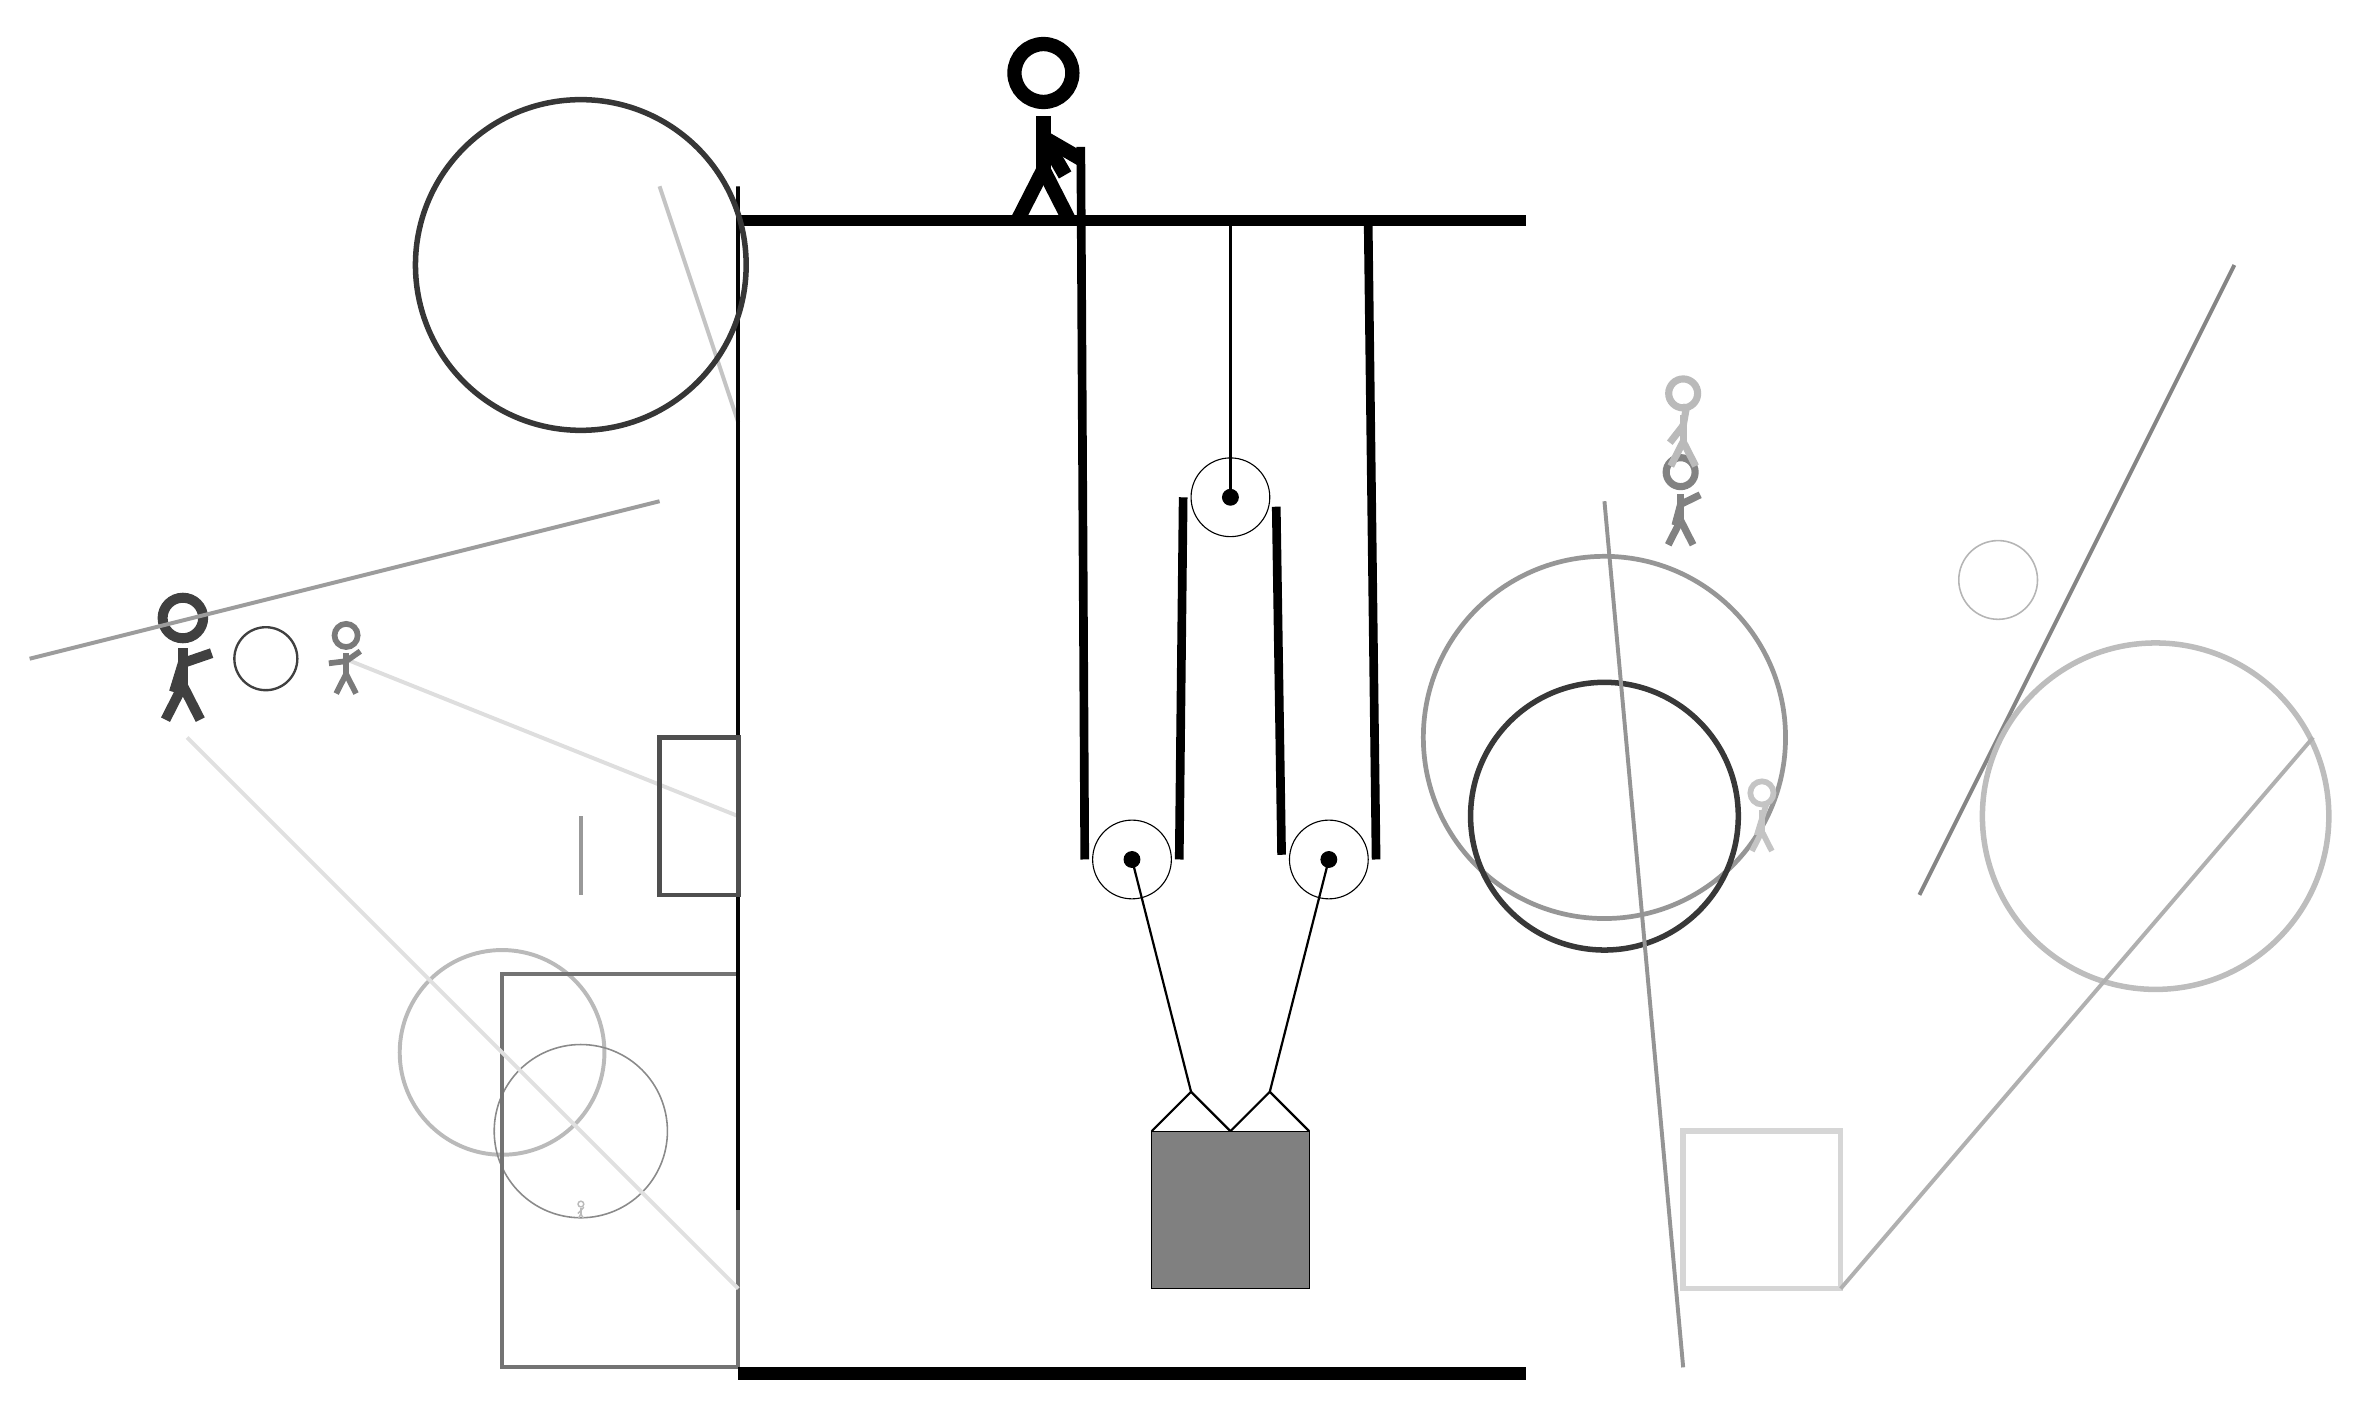
\begin{tikzpicture}
			%%%%% START %%%%%
			
			\draw[fill=black] (-4, 11.5) rectangle (6, 11.625);
			
			\draw (1, 3.45) circle (0.5);
			\draw[fill=black] (1, 3.45) circle (0.1);
			
			\draw (2.25, 8.05) circle (0.5);
			\draw[fill=black] (2.25, 8.05) circle (0.1);
			\draw[thick] (2.25, 8.05) -- (2.25, 11.5);
			
			\draw (3.5, 3.45) circle (0.5);
			\draw[fill=black] (3.5, 3.45) circle (0.1);
			
			\draw[thick] (3.5, 3.45) -- (2.75, 0.5);
			\draw[thick] (1, 3.45) -- (1.75, 0.5);
			\draw[thick]  (1.25, 0) -- (1.75, 0.5) -- (2.25, 0);
			\draw[thick]  (2.25, 0) -- (2.75, 0.5) -- (3.25, 0);
			\draw[fill=black!50] (1.25, 0) rectangle (3.25, -2);
			
			\draw[line width=1.1mm] (0.35, 12.5) --  (0.4, 3.45);
			\centerarc[line width=1.1mm](1, 3.45)(180:360:0.6);
			\draw[line width=1.1mm] (1.6, 3.45) -- (1.65, 8.05);
			\centerarc[line width=1.1mm](2.25, 8.05)(-20:180:0.6);
			\draw[line width=1.1mm](2.832, 7.93) -- (2.9, 3.51);
			\centerarc[line width=1.1mm](3.5, 3.45)(160:360:0.6);
			\draw[line width=1.1mm](4.1, 3.45) -- (4.0, 11.5);
			
			\node at (-0.07, 12.7) {\Strichmaxerl[10][120][-30]};
			
			\draw [line width=0.5mm, color=black!27](-7, 1) circle (1.3);
			
			\node[line width=0.3mm, color=black!49] at (8, 8) {\Strichmaxerl[5][75][26]};
			\draw [line width=0.6mm, color=black!41](7, 5) circle (2.3);
			\draw [line width=0.2mm, color=black!46](-6, 0) circle (1.1);
			\draw [line width=0.7mm, color=black!78](7, 4) circle (1.7);
			\draw[line width=0.2mm, color=black!11] (-4, 12) rectangle (-4, -3);
			\draw[line width=0.5mm, color=black!13](-4, 4) -- (-9, 6);
			\draw[line width=0.5mm, color=black!23](-4, 9) -- (-5, 12);
			\draw [line width=0.3mm, color=black!75](-10, 6) circle (0.4);
			\draw[line width=0.5mm, color=black!42](8, -3) -- (7, 8);
			
			\draw [line width=0.2mm, color=black!29](12, 7) circle (0.5);
			
			\draw[line width=0.7mm, color=black!16] (8, 0) rectangle (10, -2);
			\draw[line width=0.5mm, color=black!48](11, 3) -- (15, 11);
			
			\node[line width=0.3mm, color=black!75] at (-11, 6) {\Strichmaxerl[7][73][19]};
			\node[line width=0.3mm, color=black!27] at (-6, -1) {\Strichmaxerl[1][45][49]};
			\draw[line width=0.5mm, color=black!55] (-4, 2) rectangle (-7, -3);
			
			\draw[line width=0.5mm, color=black!12](-4, -2) -- (-11, 5);
			\draw [line width=0.7mm, color=black!26](14, 4) circle (2.2);
			\draw[line width=0.5mm, color=black!31](10, -2) -- (16, 5);
			\draw[line width=0.5mm, color=black!98] (-4, 12) rectangle (-4, -1);
			\node[line width=0.3mm, color=black!52] at (-9, 6) {\Strichmaxerl[4][7][35]};
			\draw[line width=0.6mm, color=black!69] (-5, 5) rectangle (-4, 3);
			
			\node[line width=0.6mm, color=black!23] at (9, 4) {\Strichmaxerl[4][73][73]};
			\draw[line width=0.5mm, color=black!39](-5, 8) -- (-13, 6);
			\draw[line width=0.5mm, color=black!40] (-6, 4) rectangle (-6, 3);
			
			\draw [line width=0.7mm, color=black!79](-6, 11) circle (2.1);
			\node[line width=0.6mm, color=black!27] at (8, 9) {\Strichmaxerl[5][52][80]};
			
			\draw[fill=black] (-4, -3) rectangle (6, -3.15);
			
			%%%%% END %%%%%
		\end{tikzpicture}
	\end{figure}	
\end{document}